

\newcommand{\doi}[1]{\def\@doi{#1}}
\documentclass[9pt,twocolumn,twoside,notitlepage]{article}
\usepackage{graphicx,xcolor}
\usepackage{listings}
\usepackage{minted}
\usepackage{amsmath}
\usepackage[colorlinks]{hyperref}
\title{UW Toroidal Shell: Moment of Inertia about z axis}
\begin{document}
%New colors defined below
\definecolor{codegreen}{rgb}{0,0.6,0}
\definecolor{codegray}{rgb}{0.5,0.5,0.5}
\definecolor{codepurple}{rgb}{0.58,0,0.82}
\definecolor{backcolour}{rgb}{0.95,0.95,0.92}
%Code listing style named "mystyle"
\lstdefinestyle{mystyle}{
  backgroundcolor=\color{backcolour},   commentstyle=\color{codegreen},
  keywordstyle=\color{magenta},
  numberstyle=\tiny\color{codegray},
  stringstyle=\color{codepurple},
  basicstyle=\ttfamily\footnotesize,
  breakatwhitespace=false,         
  breaklines=true,                 
  captionpos=b,                    
  keepspaces=true,                 
  numbers=left,                    
  numbersep=5pt,                  
  showspaces=false,                
  showstringspaces=false,
  showtabs=false,                  
  tabsize=2
}
%"mystyle" code listing set
\lstset{style=mystyle}

\twocolumn[
  \begin{@twocolumnfalse}
    \maketitle
  \end{@twocolumnfalse}
  ]


\textbf{Problem: }
Moment of inertia about z axis computed for torodial shell with major radius 1 and minor radius 0.1.
$$\iint_S  x^2 + y^2 \,dS$$
where S is defined by :\newline $f(x,y,z)=\sqrt{x^2+y^2}-1)^2+z^2 - 0.1^2=0$
 \begin{figure}[htbp]
 \centering
 \fbox{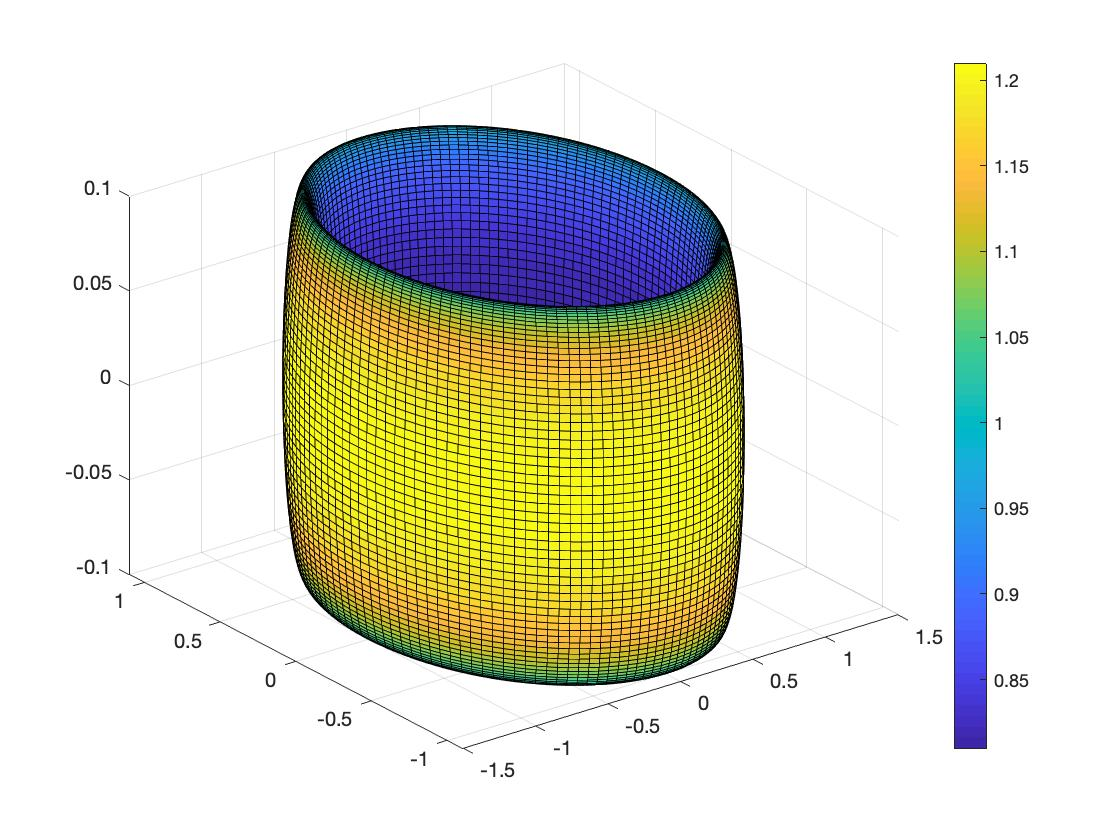
\includegraphics[width=.8\linewidth]{networks/scitile/uw_toroidal_shell/docs/toroidal_shell_moment.jpg}}
 \caption{Toroidal shell, $R= 1$, $r=0.1$, Color represents $g(x,y,z)=x^2+y^2$}
 \end{figure}

\textbf{Solution steps:}\newline
1. create a grid of points in the x,y,z plane \newline
2. compute $f$ and $g$ on all points on the grid\newline
3. compute $\sqrt{\nabla f \cdot \nabla f}$\newline
4. compute $\nabla g \cdot \nabla \chi (f)$\newline
5. compute $\rho = -1 * g * \frac{\nabla g \cdot \nabla 
\chi}{\sqrt{\nabla f \cdot \nabla f}}$ \newline
6. compute $(\sum \rho)*\delta^3$\newline
\\[4in]
{\normalfont\sffamily\bfseries\scshape\fontsize{12}{14}\selectfont \textcolor{olive} {PlaidML EDSL implementation:}}\newline
\hyperlink{https://github.com/plaidml/plaidml/tree/master/networks/scitile}{https://github.com/plaidml/plaidml/tree/master/networks/scitile}
\begin{lstlisting}[language=Python, caption= EDSL Sample Code]
def partial(F, wrt, delta):
    F_neg = -F
    dims = edsl.TensorDims(3)
    x, y, z = edsl.TensorIndexes(3)
    F.bind_dims(*dims)
    O = edsl.TensorOutput(*dims)
    if wrt == 'x':
        O[x, y, z] = F[x + 1, y, z] + F_neg[x - 1, y, z]
    elif wrt == 'y':
        O[x, y, z] = F[x, y + 1, z] + F_neg[x, y - 1, z]
    elif wrt == 'z':
        O[x, y, z] = F[x, y, z + 1] + F_neg[x, y, z - 1]
    return O / (2.0 * delta)
\end{lstlisting}
\begin{table}[htbp]
\centering
\begin{tabular}{ccc}
\hline
backend & device & runtime \\
\hline
CUDA  & GeForce GTX 1070  & 0.0069 \\
plaidml2 + opencl & GeForce GTX 1070 & 0.0112 \\
plaidml2 + LLVM  & 2.6 GHz Intel Xeon E5-2670 & 0.2774 \\
plaidml2 + LLVM  &  2.6 GHz Intel Core i7 & 0.0933\\
plaidml2 + opencl & AMD FIJI & 0.0413 \\
plaidml2 + opencl & AMD GFX906 & 0.0235\\
plaidml2 + metal & AMD radeon pro 560x & 0.0552 \\
plaidml2 + metal &  Intel UHD graphics 630 & 0.0597 \\
\hline
\end{tabular}
  \label{tab:shapefunctions}
\end{table}

\end{document}
